% THIS IS SIGPROC-SP.TEX - VERSION 3.1
% WORKS WITH V3.2SP OF ACM_PROC_ARTICLE-SP.CLS
% APRIL 2009
%
% It is an example file showing how to use the 'acm_proc_article-sp.cls' V3.2SP
% LaTeX2e document class file for Conference Proceedings submissions.
% ----------------------------------------------------------------------------------------------------------------
% This .tex file (and associated .cls V3.2SP) *DOES NOT* produce:
%       1) The Permission Statement
%       2) The Conference (location) Info information
%       3) The Copyright Line with ACM data
%       4) Page numbering
% ---------------------------------------------------------------------------------------------------------------
% It is an example which *does* use the .bib file (from which the .bbl file
% is produced).
% REMEMBER HOWEVER: After having produced the .bbl file,
% and prior to final submission,
% you need to 'insert'  your .bbl file into your source .tex file so as to provide
% ONE 'self-contained' source file.
%
% Questions regarding SIGS should be sent to
% Adrienne Griscti ---> griscti@acm.org
%
% Questions/suggestions regarding the guidelines, .tex and .cls files, etc. to
% Gerald Murray ---> murray@hq.acm.org
%
% For tracking purposes - this is V3.1SP - APRIL 2009

\documentclass{acm_proc_article-sp}

\makeatletter
\let\@copyrightspace\relax
\makeatother

\usepackage{tabularx}
\usepackage{url}
\usepackage{graphicx}
\usepackage{subfig}

\begin{document}

\title{Accountability and Privacy in the Modern Internet}
\subtitle{Comsys Seminar Paper WS 2015/16}

\numberofauthors{1}
%\author{
%\alignauthor
%Lucas Braun\\
%	RWTH Aachen University \\
%       \email{lucas.braun@rwth-aachen.de}
%}

\maketitle
\begin{abstract}
When discussing flaws in the design of the Internet, the lack of accountability and privacy mechanisms is a recurring subject matter. It is easy to argue why either of them should be a fundamental part of the world wide network, but still both are only provided in a limited manner by high level extensions. This work looks at the problems that arise from this situation and examine proposals to fix them. Furthermore, not only solutions granting either accountability or privacy are highlighted, but also how to balance between the two by replacing source addresses like they are used in IP into a return address and an accountability address, thus separating sender identity from accountability.
\end{abstract}

\section{Introduction}
The history of the modern Internet as we know it today goes back as far as the early eighties -- IPv4, ICMP and TCP, which where all specified in 1981, together with 1984's DNS, still are the foundation on which all Internet traffic is being transported.

The way these technologies are designed is heavily reflecting the challenges that were of importance at that time -- namely "the creation of a distributed communication network that is robust against packet loss and other network failures; support across multiple types of networks and communication services; and the management of Internet resources in a cost-effective and distributed way" \cite{mot}.

As the Internet began to grow bigger and bigger, new challenges that where not incorporated into these original design goals arose. The following work will focus on two of the biggest of those:
\begin{itemize}
	\item \textbf{Accountability} -- While there is certainly more to accountability in the Internet, in the context of this work it will be the possibility to hold someone (usually the sender) liable for packets in the network without a doubt. This especially implies that source addresses can not be spoofed. Furthermore, malicious and unwanted traffic should be suppressible in an accountable Internet.
	\item \textbf{Privacy} -- Privacy always means that some information is hidden from distinct parties. In the usual case that means that communication is resistant to eavesdropping, making all exchanged information unavailable to third parties. But it can also include not revealing sender identity to receivers, being part of an anonymity set or combinations of all these or more, depending on individual privacy needs.
\end{itemize}

While there is already a plethora of technologies in use that enable for varying levels of privacy, e.g., Tor (formerly known as \emph{The Onion Routing (TOR)}) and \emph{Network Address Translation} (NAT), accountability is on a completely different page. Not only is accountability hard to guarantee, but it tends to be mutually exclusive with privacy. This is largely due to the fact that the first usually means strengthening sources addresses (e.g. by replacing IP addresses with self-certifying cryptographic addresses as we will see in section \ref{sec:aip}) while the latter usually means weakening them (e.g. by only letting the network know an anonymity set a host is part of, as in NAT) \cite{apip}.

Most online traffic is of good nature. But unfortunately this is not always the case: spam is a prominent example we all know from our mailboxes and most have experienced not being able to access a favorite webpage due to denial of service attacks from botnets. A big enabler for malicious actions like that is the lack of accountability in the Internet we have right now. Given the necessary resources, attackers can spoof their IP address, making it hard to identify them and even harder to punish them. It becomes clear that accountability is not necessarily or mainly a technical consideration, but bleeds heavily into the realms of social interaction and law. Section~\ref{sec:acc} will further examine ways to make hosts liable for their actions.

When on the other hand we look at privacy, there are good reasons why the average Internet user should want and should have a reasonable level of privacy, which usually comes with anonymity or encryption. If everyone is able to gather arbitrary information about every other's Internet usage this can and will have consequences such as health insurances adjusting their premium according to search history or restrictions to free speech, for example if you are not able to speak out against a corrupt regime out of fear to be identified. In section~\ref{sec:priv} this will be discussed in greater detail and common privacy techniques will be highlighted.

But what if we want the best of both worlds? A topic rarely touched yet is how accountability and privacy can be provided at the same time. The main focus of this work will be on the \emph{Accountable and Private Inter Protocol} (APIP), which tries to find a balance between the two (see section~\ref{sec:apip}) \cite{apip}. In IP, the source address is heavily overloaded with functionalities: it not only serves as a return address for the receiver of a packet, but it is also used to identify a sender, for error reporting, deriving flow ID and for very basic accountability techniques like \emph{Unicast Reverse Path Forwarding} (uRPF). The idea behind APIP is to replace the source address with two addresses which divide the source addresses duties between each other: a return address that is only used by the receiver of a packet and can be masked from the rest of the network or even be omitted if not needed and an accountability address that points to a delegate that fulfills all the remaining duties.

The rest of this work is organized as follows: In section~\ref{sec:acc}, we discuss accountability in general and introduce the \emph{Accountable Internet Protocol} as an example of how accountability can be integrated into the network. In section~\ref{sec:priv} we do the same for privacy, using \emph{Tor instead of IP} as well as \emph{Lightweight Anonymity and Privacy} as examples. Section~\ref{sec:apip} introduces the \emph{Accountable and Private Internet Protocol} in depth. Finally, we conclude in section~\ref{sec:con}.

%To delve deeper into these topics, section~\ref{sec:acc} explains what accountability is, why it is needed and by whom and present some recent research projects while section~\ref{sec:priv} does the same for privacy. Furthermore, section~\ref{sec:apip} presents the \emph{Accountable and Private Internet Protocol}, a recent attempt at creating a solution that balances between accountabilty and privacy \cite{apip}.

%%
%% ACOUNTABILITY
%%

\section{Accountability}
%\cite{mirkovic}
\label{sec:acc}
A lot of crime and chaos in the real world is being prevented because we have mechanisms in place that associate distinct persons or groups of persons with actions, making everyone accountable for most of their actions. The Internet, as we have it today, is partly devoid of such mechanisms. While legislation is in place and it is technically possible to log wrongdoers' IPs and identify them with their ISPs' help, there are ways around that. Techniques like source IP spoofing can potentially grant attackers (that control a large enough part of the network) anonymity and enable for malicious actions such as denial of service attacks without having to fear any consequences.

Naylor et al. \cite{apip} define three key properties that must be fulfilled in an accountable Internet:

\begin{itemize}
\item For every packet there exists an entity that takes responsibility if the packet is of malicious nature
\item If a malicious flow is detected, it can be stopped quickly
\item Subsequent mischief can be prevented by punishment or expulsion
\end{itemize}

Accountability would thus be a welcomed trait in the Internet, as it can greatly help to stop and even prevent attacks. What is needed to provide such accountability is some efficient way to verify the alleged identity of a source, something that is not done directly on the network layer of today's Internet. 

But accountability is not only interesting in the light of malicious attacks; without accountability it is hard to securely identify why and because of whom network errors are caused. If this was changed, it could enable ISPs to trace out liabilities far more exact and at the same time force them to try harder to fulfill them \cite{mot}. 

Approaches to fix the lack of accountability in the Internet do exist, but many of them come with their own shortcomings, rendering them not ideal for real world deployment. For example they rely on complicated mechanisms changing "the free-access model of the Internet", external sources of trust, or on manual filtering by network operators \cite{aip}.
%TODO: examples for this, maybe from AIP?

As an example of how accountability can be implemented into the Internet we will now introduce the \emph{Accountable Internet Protocol}.

%With IPA, \emph{IP made Accountable}, Li et al. propose using DNSSEC as a lightweight PKI \cite{bootstrapping} 

\subsection{Accountable Internet Protocol}
\label{sec:aip}
Andersen et al. propose the \emph{Accountable Internet Protocol} (AIP) \cite{aip} as a replacement for the current \emph{Internet Protocol} (IP). Hosts and domains using AIP are enabled to prove their identity without the need for an external trusted authority. While their approach certainly is not the be all and end all, it has gained a lot of popularity and spawned plenty followers\footnote{Cited 75 times by October 2015}.

In AIP, packets sent by end hosts get intercepted at the first-hop router for verification. Traditional addressing is replaced by a cryptographic key which is used to unmistakably link packets to end hosts and thus prevents techniques like source address spoofing. Additionally to the verification at the first-hop, receivers can stop unwanted network flows by sending a special shut-off packet that is processed directly by the network interface card, which then suspends packets from being sent to the specific receiver.

\subsubsection{Basic design}
\label{sec:aipbd}

In AIP, the transition to complex prefixed IP based addressing schemes is reverted in favor of flat (and thus simpler), self-certifying multi component address. The usage of IP addresses gets completely removed and addressing is solely done over AIP as follows: Each independently administered network -- typically that is the network of an ISP -- gets divided into one or more \emph{accountability domains} (ADs) by its administrative unit, providing each AD with a globally unique identifier. Likewise, every end host must be provided with a globally unique EID identifier, leading to an address scheme of \texttt{AD:EID}. In case accountability domains are hierarchically organized, the scheme can be extended to \texttt{AD$_1$:AD$_2$:\ldots:AD$_k$:EID}. Furthermore, if a host connects to an accountability domain via multiple network interfaces, each interface is provided its own EID by altering the \emph{interface bits} -- the last eight bits of the EID.

\begin{figure}[h!]
	\newcolumntype{C}{>{\centering}X}
	\begin{tabularx}{0.47\textwidth}{|c|C|c|}
		\hline & & \\
 		Crypto vers & Public key hash & Interface \\
		8 bits & 144 bits & 8 bits \\ & & \\
		\hline
	\end{tabularx}
	\caption{AIP addresses consist of a version number, a hash of a public key and an interface identifier (which is set to zero for accountability domains) \cite{aip}}
	\label{fig:aipadr}
\end{figure}

This simplification of the addressing enables for \emph{self-certifying} addresses: the main part of the 160 bit long AIP address is simply a 144 bit long hash of the endpoint's respective accountability domain's public key (Figure \ref{fig:aipadr}). The remaining 16 bits are divided into 8 bits denoting the version of AIP used (to cater for the need of improved cryptography methods when existing methods get weakened) at the beginning of the address and the aforementioned 8 bit interface identifier at the end.

\subsubsection{Verification}
\begin{figure}[t]
  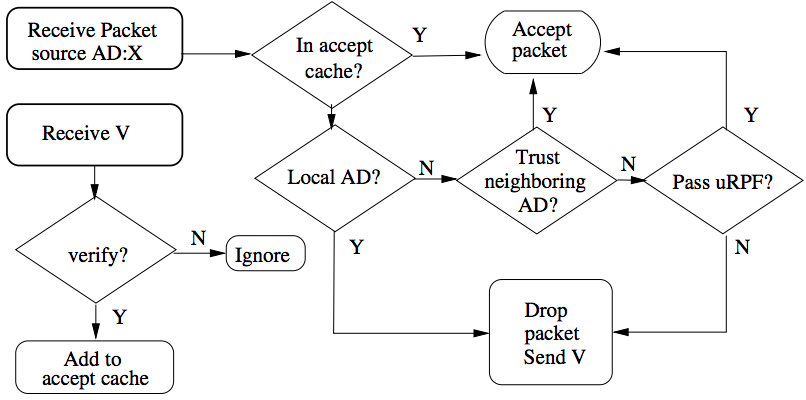
\includegraphics[width=0.5\textwidth]{images/aipflow.PNG}
  \caption{Flowchart showing the process for verifying a packet's source address \cite{aip}}
  \label{fig:aipflow}
\end{figure}
The verification process in AIP is shown in figure \ref{fig:aipflow}: When an end point tries to send a packet, it is the first-hop router's duty to verify the end point's identity. When a packet from a not-verified host arrives, the packet is dropped and the router replies with a \emph{verification packet} V. This packet is signed with a periodically created router specific secret. If the host that receives V has originally sent the packet (to verify this, hosts keep hashes of recently sent packets), it signs this packet with its private key and returns it to the router, which can now verify the sender's identity with the help of his public key and permits the sender to resend the dropped packet as well as subsequent packets.

As packets transit from AD \emph{A} to AD \emph{B}, the latter must decide whether he trusts \emph{A} to have correctly verified the packet. If \emph{B} does not initially trust \emph{A}, he performs an \emph{Unicast Reverse Path Forwarding} (uRPF) check. Should this fail as well, the router in \emph{B} drops the packet and verifies it with the source as if it was the sources first-hop router (see Figure \ref{fig:aipflow}).\looseness=1
%TODO: shortly explain uRPF

\subsubsection{Shut-Off}
In addition to AIP's inherent protection against source address spoofing, flooding attacks can be stopped by sending a \emph{shut-off packet} (SOP) to source hosts. Under the assumption that most flooding attacks are coming from compromised hosts and are not initiated by the legitimate owners of these hosts, smart network interface cards can install a filter blocking the malicious packets for an amount of time specified by the victim in its initial SOP.\looseness=1

\subsubsection{Verdict}
AIP sure provides strong accountability to the network, but there are also drawbacks. Since senders are cryptographically linked to their packets' source addresses, privacy is worse if compared to traditional IP. Furthermore, the need for special smart network interface cards to support shut-off functionality is an unnecessary barrier in the design. The approach presented in section~\ref{sec:apip} will show how the concept of AIP can be extended to overcome these shortcomings without weakening the provided accountability mechanisms.\looseness=1

%%
%% PRIVACY
%%

\section{Privacy}
\label{sec:priv}
Privacy (in general, but especially) in the Internet has increasingly come into the spotlight during the past years. Even more so since the global surveillance disclosure in the year 2013, initiated by whistle blower Edward Snowden, which has unprecedentedly shown the real dimensions surveillance has grown to.

The "I've Got Nothing To Hide" argument often heard in this context is a fallacy that stems from the misunderstanding that privacy is the hiding of a wrong \cite{solove}. Imagining an Internet without privacy, it would for example be conceivable that health insurances higher their premium for insurance holders who look up certain diseases or, say, order a book on cancer in one week and a wig in the next one.

Mechanisms to protect a users privacy on a network level are manifold and so are their modes of operation. Most of them focus on the two main characteristics of privacy: anonymity and security. Anonymity is granted when an entity is unidentifiable within other entities, building an \emph{anonymity set}. Security, on the other hand, requires the data sent over a network to be masked from eavesdroppers, which is usually done via encryption. Solutions that provide either one or both of these characteristics exist; Some more commonly used are the following:

\begin{itemize}
\item \textbf{Proxy servers} let you route traffic over them, which will hide your IP address from simple checks but do not provide any privacy beyond. This is probably the most lightweight solution -- since the proxy server is not providing any encryption and is really just rerouting traffic to make it look like it is coming from the proxy, a single proxy can typically serve thousands of clients. They come in different flavors: very fast HTTP proxies that only accept HTTP traffic and the more generic SOCKS proxies, which are a little bit slower but accept arbitrary types of traffic.
\item \textbf{Virtual Private Networks} (VPNs) provide a fully encrypted tunnel to the Internet and thus potentially provides a high level of privacy. They can however be slow and ultimately the user's privacy depends largely on the discretion of the VPN provider. The best VPN does not help boosting your privacy at all if it keeps logs about all the traffic you tunnel through and makes these logs available to a third party. 
\item \textbf{Onion Routing} redirects traffic over a random route of proxies, accessed over so called rendezvous points. The data is encrypted several times by the client and each proxy \emph{peels off} one encryption, like the layers of an onion. Figure \ref{fig:tor} shows an example of this, where the initial message gets encrypted three times by the sender. Than Router A, Router B and Router C each decrypt one of the layers, so that the message reaches its destination unencrypted. Analogously, responses are getting encrypted once by each proxy and can than be decrypted by the client. Onion Routing, while a little bit slow, is considered relatively secure. Research has unveiled quiet a few possible attacks and weaknesses, many of which are based on controlling the first and the last proxy in an onion route. A popular example implementation of onion routing is Tor. This technology is currently considered to provide the maximum amount of privacy possible for private persons.
\item \textbf{Network Address Translation} (NAT) was originally developed to fight the scarcity of IP addresses. A router that is part of two networks can translate IP addresses in packet headers from the address space in the first network to a different address in the second network. If the router now for example maps many different addresses from the one network to a single address on the other, it thereby creates an anonymity set providing some degree of privacy its endhosts.
\end{itemize}
%TODO: quotations for all of this :(

\begin{figure}[t]
  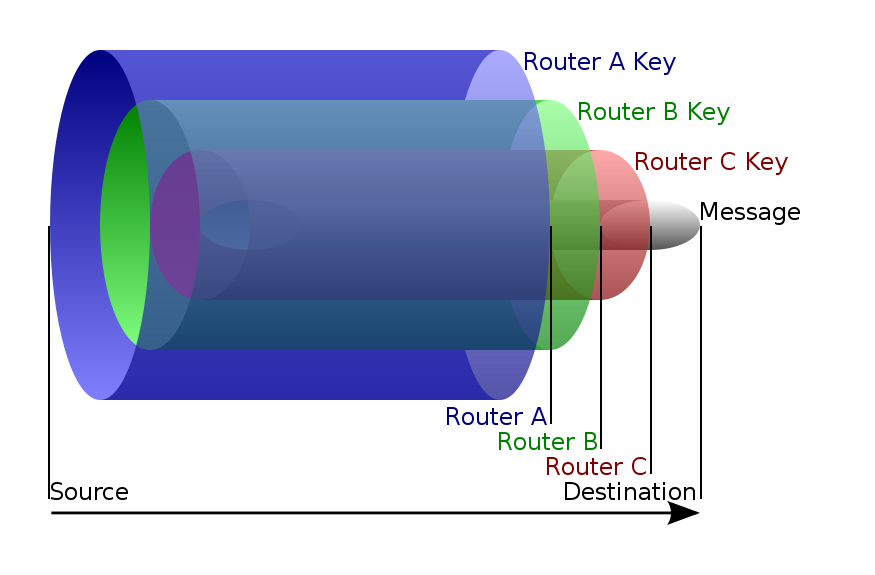
\includegraphics[width=0.5\textwidth]{images/tor.png}
  \caption{Visualisation of onion routing. At the source, the message starts with three mutually distinct encryptions. Then, each onion router that the packet passes peels off one encryption so that at the destination all onion routing related encryptions have been removed. \cite{tor-dia}}
  \label{fig:tor}
\end{figure}
Apart from these examples which are readily available for everyone who wants to increase their privacy in the Internet that have today, the question about how to improve the flawed design of the underlying network has been in the focus of many research projects in the past years. We are still far away from an ultimate answer, but the following examples might give an idea of the direction we are moving.
\subsection{Tor instead of IP}
Liu et al. propose using Tor not on top of IP, but instead of IP \cite{tor}. In their approach, ISPs still build the foundation of the network, each managing its own domain and relationships to each other. What differs from the traditional Internet is that the \emph{Border Gateway Protocol} (BGP) gets replaced by onion routers and rendezvous mailboxes, what leads to all communication on the network being over onion routes, without exception.

ISPs advertise pathlets \cite{pathlet} of the form \texttt{<ingress ISP, transit ISP, egress ISP>} for pairs of neighboring ISPs. End hosts then define a path for their packets using these triplets and a mailbox address. The actual onion routing is done by zigzagging in the so called core network, which consists only of the biggest ISPs (Tier 1 and some Tier 2), which can handle the bandwidth overhead better than smaller ISPs. Packets that do not need anonymity simply do not zigzag in the core.

While this approach provides a high amount of anonymity to every host on the Internet, this is probably also its biggest drawback. It disposes the Internet of any accountability mechanism and makes censorship hard, two traits that are unlikely to persuade ISPs and governments to deviate from IP, thus leaving Tor instead of IP to be a neat thought experiment.

Furthermore, the same performance limitations that hold true for Tor are also applicable here. While overhead can be kept minimal by not zigzagging in the core, doing so for improved privacy will always introduce noticeable latency.
\subsection{Lightweight Anonymity and Privacy}
To close the gap between systems that provide slow but strong anonymity -- like Tor or mix networks -- and zero latency systems that do not provide anonymity, Hsiao et al. propose \emph{Lightweight Anonymity and Privacy} (LAP) \cite{lap}. The authors aim for masking the identity against servers (rather than globally, as Tor, etc. do) while introducing as little latency as possible in return. 

LAP uses encrypted paths, which they call \emph{e-paths}, instead of source and destination addresses; the first-hop router encrypts the source address and the egress interface's address and forwards it. The next hop router encrypts his ingress and egress address, appends the encrypted information to the e-path and forwards it. This procedure is repeated until the destination host is reached and the established route can then be used for packet forwarding. The level of anonymity granted (and with it the resulting latency) depends on the length of the e-path. Hosts can use the header field HTE (Hop To Encrypt) to regulate how many hops should be encrypted.

LAP is good at what it is designed for -- granting users anonymity to everyone but the own ISP -- and does so in a fast enough and uncomplicated way to qualify as an always on solution and the authors even describe how it can be deployed on top of IP. However, in use cases where anonymity against the own ISP plays a role, LAP is not applicable.

%\subsection{BLIND}
%\cite{blind}  

%%
%% APIP
%%

\section{Accountable and Private Internet Protocol}
\label{sec:apip}
\begin{figure}[t]
  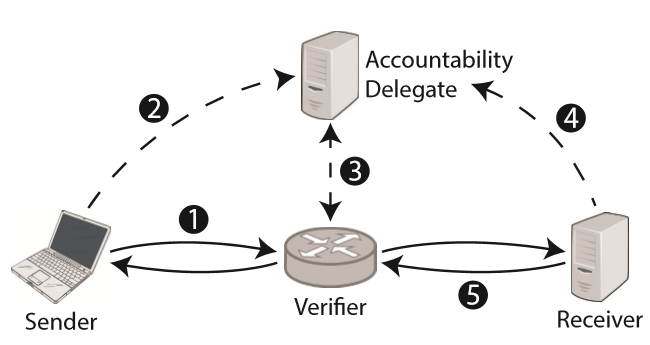
\includegraphics[width=0.48\textwidth]{images/apipoverview.PNG}
  \caption{A High-Level overview of APIP. (1) The sender sends a packet with at least the accountability address filled out and if needed also a return address (which can be masked). (2) At the same time, the sender also briefs its accountability delegate about the sent packet. (3) On-path routers may check with the accountability delegate whether the packet is being vouched for by him and drop it otherwise. (4) Malicious flows can be reported to the corresponding delegate, who will then stop verifying packets belonging to the reported flow. (5) If packets await an answer, the receiver can demask the return address and use it as the destination address in its answer. \cite{apip}}
  \label{fig:apipoverview}
\end{figure}
With the \emph{Accountable and Private Internet Protocol} (APIP) \cite{apip}, as the name suggests, Naylor et al. try to find a way to balance between the seemingly mutually exclusive properties accountability and privacy. To achieve this goal they borrow heavily from AIP (see section \ref{sec:aip}), but delegate the job of verifying identities to so called \emph{accountability delegates}. The way this is done opens up the possibility to mask ones return address and thus allows for the application of privacy preserving methods like end-to-end encryption and NAT. A very high-level overview of this is giving in figure \ref{fig:apipoverview}: When a host sends a packet (1), he also briefs his accountability delegate about the packet he just sent (2). On-path routers can now verify the authenticity of packets by asking the corresponding accountability delegate if he does indeed vouch for the packet (3). When the packet reaches the receiver, he can decide whether he wants to reply to the packet (5) or ask the delegate to no longer vouch for packets between this sender and receiver by sending a shutoff message the delegate (4).

The authors argue that the way source addresses are used today creates an unnecessarily heavy overload. The roles they identify for the source address are:

\begin{itemize}
\item \textbf{Return Address} Its used as the destination in response packets
\item \textbf{Sender Identity} Its used to track users on an application level
\item \textbf{Error Reporting} Its used for routing ICMP error messages
\item \textbf{Flow ID} Its one of the five values that define a TCP/IP connection 
\item \textbf{Accountability} uRPF provides basic protection against IP spoofing and uses source addresses for this functionality
\end{itemize}

%\begin{table*}[t]
%	\label{tab:sourcerole}
%	\newcolumntype{L}{>{\left}X}
%	\renewcommand{\arraystretch}{1.5}
%	\begin{tabularx}{\textwidth}{lllX}
%		\hline 
 %		\textbf{Role} & \textbf{Where Used} & \textbf{Layer} & \textbf{Comments} \\ \hline
%		\emph{Return Address} & Destination & Transport & Not needed for routing to the destination, only used by the destination in response packets \\
%		\emph{Sender Identity} & Destination & Application & Not really done anymore, some webpage still do this to track users across sessions \\
%		\emph{Error Reporting} & Routers & Network & Used as a destination for ICMP error messages \\
%			& Destination & Network & \\
%		\emph{Flow ID} & Destination & Transport & Used by end-hosts to demultiplex flows \\
%			& Routers & Network & Routers distinguish flow for traffic monitoring and engineering \\
%		\emph{Accountability} & Routers & Network & More elaborate protocols like AIP use cryptographic source addresses for accountability \\
%			& Destination & Network & It must be possible to identify and shut down a malicious flow \\
%		\hline
%	\end{tabularx}
%	\caption{The roles a source address plays and where each is used \cite{apip}}
%\end{table*}

Accountability, as we have seen, usually comes with a strengthened source address while privacy implicates weakened or masked source addresses. The basic idea that enables APIP to cater the needs of both functionalities is now that, in order to successfully route a packet to its destination, the return address role is never used and can thus be separated from the rest. To achieve this, the source address gets split into an accountability address and a return address. It is now no longer necessary to know who sent a packet in order to be able to verify that it is accounted for, since verification is done exclusively with the help of the accountability delegate.

\subsection{Addressing and packet flow}
%\begin{figure}[h]
%  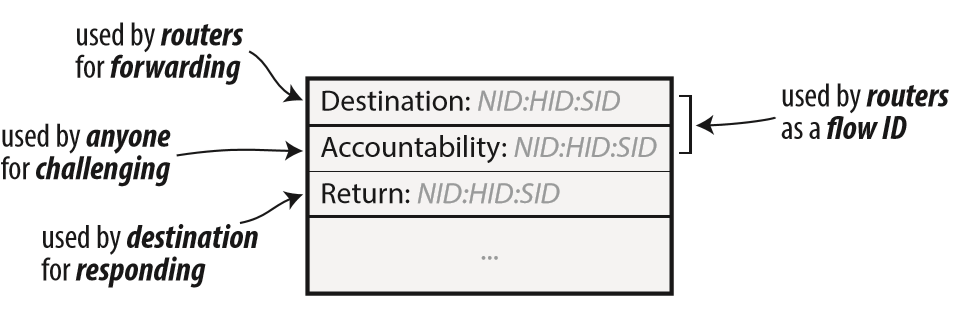
\includegraphics[width=0.5\textwidth]{images/apipaddressing.PNG}
%  \caption{In APIP, traditional souce addresses are split into a public accountability address (pointing to an accountability delegate) used for routing and verifying packets, and a return address pointing to the actual sender of the packet. That makes the return address optional and maskable. \cite{apip}}
%  \label{fig:apipaddressing}
%\end{figure}

In APIP, addresses are always made up of the following components:

\begin{itemize}
\item \emph{network id} (\texttt{NID}): used to identify the domain the host resides in
\item \emph{host id} (\texttt{HID}): used to find the host inside of it's domain. The \texttt{HID} is assumed to be self-certifying, as explained in section \ref{sec:aipbd}
\item \emph{socket id} (\texttt{SID}): to further specify the host's socket used for the packet
\end{itemize}

A full address then has the form \texttt{NID:HID:SID}.

Notice that this doesn't make any assumptions about the underlying protocol, but rather is a generic addressing scheme which is applicable to most protocols. For example, when applied to IP, \texttt{NID} and \texttt{HID} are represented by an IP address while \texttt{SID} corresponds to the port number. However, the assumption about the \texttt{HID} being self-certifying must be relaxed to accommodate APIP with IP, which in turn leads to the need for a Public-Key-Infrastructure. 

Depending on it's type, each packet uses either two or three APIP addresses. The two mandatory ones are the \emph{destination address} and the \emph{accountability address}, which is pointing to the accountability delegate. The optional third address is the \emph{return address}, which is used if a response to the packet is expected and is not needed otherwise.

An implication of this approach is that flow IDs (the 5 tuple used to identify related messages in a network) might not be fine granular enough if a single accountability delegate vouches for several clients, but this can be fixed by either using distinct SIDs for every client and/or by adding a flow ID field to the packet header. How this is handled does have an impact on both privacy and flow control; while just allocating the same flow ID to every client might provide maximum anonymity, it can also lead to a lot of non-malicious traffic being blocked when only a single client misbehaves. Then again, assigning a unique flow ID to every client might provide very fine flow control but it also makes it easy to map traffic to specific senders. A good trade off between these extremes is posed by assigning each client not a single unique flow ID but a pool of enough flow IDs to ensure a sufficient level of anonymity. 

\subsection{Accountability mechanism}

The process of verifying packets is somewhat similar to AIP, but additionally uses a level of indirection: When sending a package, the sender also informs it's accountability delegate about said package by calling the delegate's \texttt{brief(packet, clientID)} interface. Any on-path router as well as the packet's receiver can act as a verifier by calling the delegate's \texttt{verify(packet)} interface. Verifiers are than free to filter traffic that can not be verified and furthermore receivers can use the delegate's \texttt{shutoff(packet)} interface to permanently keep the delegate from vouching for a specific flow. We will now describe how \texttt{brief}, \texttt{verify} and \texttt{shutoff} work.

\subsubsection{Brief()}
\begin{figure}[!tbp]
  \centering
  \subfloat[Fingerprint Collection]{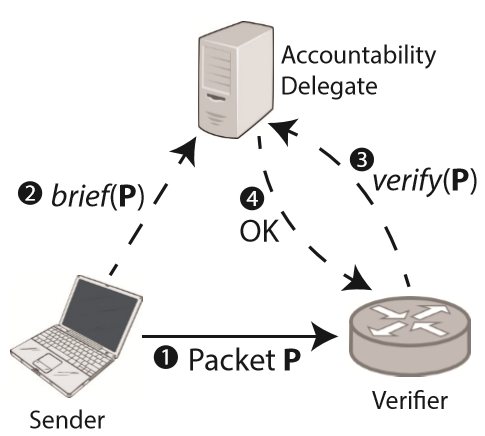
\includegraphics[width=0.23\textwidth]{images/briefing-finger.PNG}\label{fig:briefa}}
  \hfill
  \subfloat[Recursive Verification]{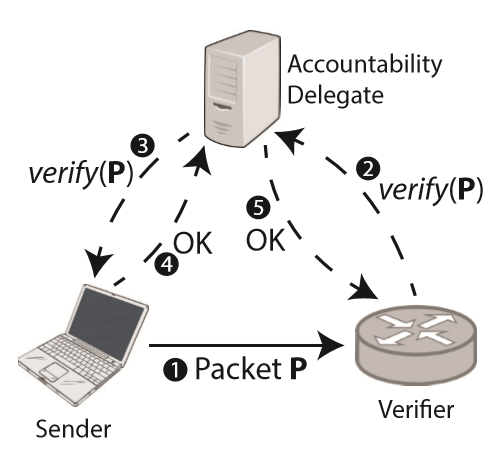
\includegraphics[width=0.23\textwidth]{images/briefing-recursive.PNG}\label{fig:briefb}}
  \caption{The two briefing techniques in APIP \cite{apip}}
\end{figure}
The briefing mechanism can be seen in Figure \ref{fig:briefa}. Informing the accountability delegate about new packets is done by either briefing each packet individually with the transmission of the packet's fingerprint or by periodically briefing them in bulk with the transmission of a bloom filter of several fingerprints (2). Verification is done directly with the accountability delegate (3 and 4) and will be described further down. The fingerprints themselves are of the following form:
\begin{equation}
F(P) = H(K_{SD_S} || P_{header} || H(P_{body} ))
\end{equation}
where $H$ is a cryptographic hash function and $K_{SD_S}$ is a symmetric key only known to the sender and the delegate.

Furthermore, clients append their client ID and a message authentication code derived from the symmetric shared secret to the brief:
\begin{equation}
\texttt{brief(P)} + clientID || F(P) || MAC_{K_{{SD}_S}}(clientID || F(P))
\end{equation}
By default every packet sent in APIP must be verifyable. To circumvent the need for verification on the briefs, a token field is included in the briefs' header. This could for example be a hash chain of a shared secret between sender and delegate which is agreed upon when the client registers with the delegate. The delegate will know in which packets it has to look for this token, since briefs' accountability and destination addresses are identical; both point to the delegate itself.

\paragraph{Recursive Verification}
Instead of using the aforementioned briefing mechanism, it is also possible to do recursive verification and merely use the accountability delegate as a middleman as shown in Figure \ref{fig:briefb}. In this case, \texttt{brief()} is not used. Instead, the delegate forwards all calls to \texttt{verify()} (2) to the packet's alleged sender (3) who in turn has to decide whether he indeed sent the packet or not and respond accordingly to the delegate (4) who then forwards the confirmation to the verifier (5). While this approach saves network and storage overhead it also has a drawback; in order for this to work, every flow ID must be mapped to exactly one client, potentially reducing client anonymity.

\subsubsection{Verify()}
When a packet passes a router, it checks whether the packet's flow ID has already been verified during the current \emph{verification interval}. At the end of each interval all verifications get purged. If it has not yet been verified, the router will verify the packet with the accountability delegate specified in the packet header by sending 
\begin{equation}
\texttt{verify(P)} = P_{header} || H(P_body) || MAC_{K_V}(P_{header} || H(P_{body}))
\end{equation}
to the delegate. The router will typically choose to drop the unverified packet and inform the sender about the ongoing verification process. The accountability delegate than checks whether the packet in question has been briefed by it's sender, the used \texttt{SID} is associated with the sender and that the connection between sender and receiver has not been blacklisted with a call to \texttt{shutoff()}. In case that all three conditions are met, the verifier gets an affirmation packet 
\begin{equation}
OK(P) = \{\texttt{VERIFIED} || \texttt{verify(P)} || K^+_{D_S}\}_{K^-_{D_S}}
\end{equation}
from the delegate and adds the flow to its whitelist for the current verification interval.

Due to how the briefing and verification process works, it makes a lot of sense for ISPs to supply their clients with accountability delegates. This way network overhead and latency for briefing is limited to a minimum and it also provides the ISP with insight on the amount of unverified traffic a client is causing.

\subsubsection{Shutoff()}
As previously mentioned, receivers can use a call to \texttt{shutoff()} to tell an accountability delegate that they do not wish to further receive transmissions from one of their clients, even if his packets are verifiable. The receiver sends a packet
\begin{equation}
\texttt{shutoff(P)} = \{P_{header} || H(P_{body}) || duration || K^+_R\}_{K^+_R}
\end{equation}
to the delegate that is vouching for packet $P$.

In addition to blacklisting and thus preventing the client from sending to this particular receiver for the given duration, the delegate may contact its client about the malicious traffic that is coming from him to work on a solution. Depending on whether the client is a victim himself (i.e., is compromised by a bot net) or was sending malicious traffic on purpose, the delegate might even withdraw from their contract and/or report him if he is breaking law. While this mechanism is primarily meant to give receivers control over the sources they want to receive data from, it makes sense to open this is up in some way to higher authorities like ISPs.

\subsection{Privacy mechanism}
In APIP, privacy is achieved by masking the return address used in the protocol's header information. Since the return address is not needed when forwarding packets, nor for APIP's accountability mechanism, various masking techniques can be applied, depending on who it shall be hidden from. While APIP does not dictate any specific techniques, the authors give two examples:
\begin{enumerate}
\item \textbf{End-to-end Encryption} hides the return address from everyone but the receiver. This could either be done directly on the network layer or be moved higher up like it is done in IPsec. 
\item \textbf{Network Address Translation} can be used to hide the sender's address not only from the network, but also from the receiver. This is not a problem since this does not affect accountability. However, it must be considered that this will narrow down the anonymity set the closer the packet is to the source and will be especially small if NAT is only done at the first hop.
\end{enumerate}
An obvious way to increase privacy in APIP is to drop the return address altogether for packets that do not necessitate them or only send it with the first packet of a flow and rely on the receiver to save it for later reuse.

\subsection{Weaknesses}
The design of APIP fixes some open problems but it also comes with its own shortcomings. The main weaknesses of APIP are found in the selection process of trustworthy delegates and the liability to verification and brief flooding. The authors offer several strategies to overcome those weaknesses but also state that they merely want to lay the groundwork for future discussion.

\subsubsection{Delegate Trust}
The shortcomings of APIP mainly stem from the dependency for trustworthy accountability delegates. A trustworthy delegate will reliably perform the following three tasks:
\begin{itemize}
\item Protect its clients' privacy
\item Verify packets that has been briefed for, and only these
\item Reacting correctly to \texttt{shutdown()} calls 
\end{itemize}
Not only can delegates gather (and possibly release) a lot of data about each of its clients' communication partners (albeit they only see the packet headers and never the packet contents), but they can also go rogue by deliberately not verifying any packets from a chosen client, effectively blocking communication for him, or by verifying packets that where not briefed for and ignoring calls to \texttt{shutdown()}.

To combat misbehaving delegates, the authors propose to have a central authority which monitors a list of trusted delegates. Verifiers should only accept packets with a whitelisted accountability address and delegates that fail to meet the authorities requirements are simply removed from the list. If the central authority is realized in a way that ensures that everyone can trust them this is an acceptable solution. If this can not be guaranteed, this approach just moves the problem without fixing it.

The alternative to allow every host to behave as an accountability delegate for itself (like in AIP) or anyone else seems to be worse, since it leaves doors wide open for botnet attacks, whose prevention are one of the main motivations of APIP. However, the authors admit that there needs to be further discussion on this topic and a feasible solution probably lies somewhere in between.

\subsubsection{Flooding Attacks}
Trustworthiness of delegates is not the only security aspect that must be considered. More precisely, APIP is prone to two different kinds of flooding attacks:
\begin{itemize}
\item \emph{Verification-Flooding} There is not really anything preventing hosts from flooding delegates with verification requests. Only the delegate can decide which requests are forged and which are honest. Delegates will need an efficient way to inform the attacker's source domain about misbehaving hosts. 
\item \emph{Brief-Flooding} In an analogous manner, clients can occupy their delegate by spamming them with briefs. To differentiate attacks from very active clients, delegates could enforce rules like only sending bloom filter periodically if their briefs reach a certain threshold. Clients then have to agree to these rules when they sign up for a delegate's service and delegates are free to cancel contracts with clients that do not comply.
\end{itemize}

\subsection{Evaluation}
\begin{table*}[t]
	\newcolumntype{L}{>{\left}X}
	\renewcommand{\arraystretch}{1.5}
	\begin{tabularx}{\textwidth}{lXXX}
		\hline 
 		& \textbf{Computational Overhead} & \textbf{Storage Overhead} & \textbf{Bandwidth Overhead} \\ \hline
		\texttt{brief()} & 2-3 hashes p.p. (per packet) & 20 bytes p.p. & 2.5\% \\ 
		\texttt{brief()} bloom filters & 2-3 hashes p.p. & one bloom filter per client & 0.25\%-0.5\% \\ 
		\texttt{verify()} & $\le$78.000 lookups in table with 1.5 million entries at a 10 second purge interval & 120 bytes per flow, $\le$94MB at a 10 second purge interval & \\ 
		\hline
	\end{tabularx}
	\caption{Computational, storage and bandwidth overhead for APIP's main functions \texttt{brief()} with and without using bloom filters, and \texttt{verify()}.}
	\label{tab:evalcomparison}
\end{table*}
When considering the use of APIP in a real world scenario, we need to know how well it performs. How much overhead does it introduce in regards of computational power, storage and bandwidth? To answer these questions, the authors took a 5 minute trace with NetFlow from the border routers of their university network, gathering ten million flows, and extrapolated APIP's overhead from this data set. Unfortunately, they only call the network 'mid-sized', without stating a specific network size. 

Table \ref{tab:evalcomparison} gives a quick overview of their findings and the following subsections will describe them in more detail.

\subsubsection{Brief()}
The overhead of \texttt{brief()} is heavily dependent on whether raw fingerprints are sent or they are being aggregated as bloom filters before being sent. Regardless, clients will have to compute two hashes needed for every fingerprint. Additionally one more hash is needed for the computation of the MAC used in the \texttt{brief()}, totaling to 2-3 hashes depending on whether bloom filters are used and if they are, how many packets get briefed with a single filter. While this very reasonable for end hosts, it might not be so reasonable anymore for big servers, which could be slowed down or even topped out by the amount of hashes that must be computed for high packet numbers. Even high performing CPUs usually do not reach 100 mega hashes per second (MH/s) \cite{hashes}, but ASICs used for mining cryptocurrencies are powerful enough to close this gap.

Since briefs are only saved at the accountability delegates, overhead will only happen there. The amount of space that is needed depends on the chosen expiration interval as well as whether bloom filters are used or not. For saving the plain fingerprints 20 bytes are needed per packet, which is the size of the corresponding SHA-1 hash. With bloom filters the demand for storage can be narrowed down to a single filter per client.

Analogously, bandwidth overhead stays much lower when bloom filters are used; an overhead of 2.5\% for sending fingerprints can be reduced to 0.25\%-0.5\% with the use of filters, assuming that a new filter is sent out every second. However, the recorded trace did not include local addresses, making filtering on a per flow basis rather than per client necessary. A real world number could thus be even lower for the variant using filters.

\subsubsection{Verify()}
Verification overhead is due to computational overhead at the delegates and storage overhead at the verifying routers. Both is dependent on the chosen verification interval: while storage overhead (and also the time until a \texttt{shutoff()} takes effect) grows with interval length, delegates get to respond to less calls to \texttt{verify()}. The gathered data suggests that an interval length of ten seconds is a good trade off, since most flows aren't longer than this (making re-verification of most flows unnecessary) and it is still short enough to keep storage requirements at verifiers reasonable.

At a ten second interval length, given the recorded trace, delegates would process $\le$78.000 \texttt{verify()}s a second, leading to that many lookups in a table with 1.5 million entries, checking for the corresponding \texttt{brief()}, and a single signature generation for signing the response each. Considering that those numbers assume that the whole university network incorporates only a single accountability delegate this sounds acceptable, but without knowledge of the exact network size it is hard to discuss this.

The storage overhead at verifiers stems from the need to maintain whitelists about flows that have already been verified. Each entry in a whitelist accommodates two host addresses of the known form \texttt{NID:HID:SID}. To comply with the assumption that addresses are self-certifying, the addresses are assumed to be three times the size of a SHA-1 hash (which is 20 bytes), leading to a size of 120 bytes per whitelist entry. For the recorded data and a ten second interval for purging the list, storage requirements are $\le$94 MB for every verifier.

\subsubsection{Shutoff()}
Since a \texttt{shutoff()} only takes effect for a specific flow after at least one whitelist on the route has been purged, the delay scales linearly with interval length and can be reduced by forcing more routers to verify traffic.

\subsection{Deploying APIP on top of IP}
\begin{figure}
  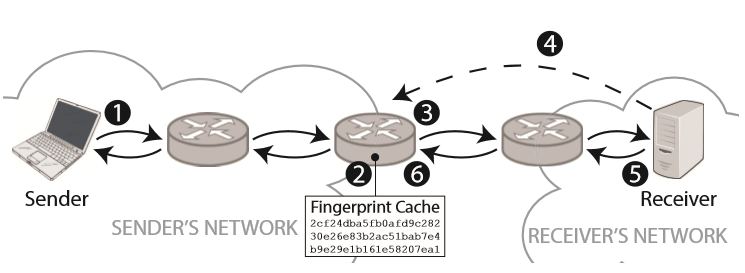
\includegraphics[width=0.5\textwidth]{images/apipoverip.PNG}
  \caption{Example design for APIP over IP: (1) APIP-unaware host sends packet as he usually would. (2) The ISP's border router saves the packet's fingerprint and (3) translates the source address. (4) Receivers use \texttt{shutoff()} when receiving malicious packets, upon which border routers react. (5) Otherwise they respond to the packet, (6) the border router translates the destination address in the response back to the original senders address and forwards it back to him. \cite{apip}}
  \label{fig:apipoverip}
\end{figure}
As mentioned before and despite its name, APIP is kept relatively generic and can be adapted to diverse carrier protocols. For a real world deployment it is the most interesting to see how it can be tailored to fit the predominant IP, a problem the authors offer a concrete design for.

The beauty of said design is that end hosts are not aware that APIP is used. They send packets as they would usually and the work is done at the domains' gateway routers. The gateway routers translate the source address of outgoing packets, masking the return address and providing a accountability address at the same time. Briefs are kept locally and calls to \texttt{verify()} and \texttt{shutoff()} are processed directly at the gateway router. Since IP addresses are not self-certifying though, cryptographic keys must come from somewhere else.

Figure \ref{fig:apipoverip} describes the way packets would take in this incarnation of APIP: The APIP-unaware host sends usual IP packets (1). When they reach the ISP's border router, the router saves the packet's fingerprint (2), translates the source address and forwards the packet (3). If a packet is unwanted, the receiver sends his \texttt{shutoff} request directly to the border router (4). Otherwise, the receiver responds to the packet as usual (5) and it gets routed back to the initial sender via NAT at the border router (6).

%%
%% OUTRO
%%

\section{Conclusion}
\label{sec:con}
This work discusses the role of accountability and privacy in the modern Internet. It explains why both are only present to a insufficient degree, why this should be changed and especially describes approaches to do so from the real world and from research. Most prominently is the idea behind APIP -- to ease the burden that source addresses have to carry and split them into a return address and an. accountability address. While the concept has to relaxed and somewhat weakened to be deployable on top of IP, the approach is sound and prepares the ground for more explicit proposals.

%
% The following two commands are all you need in the
% initial runs of your .tex file to
% produce the bibliography for the citations in your paper.
\bibliographystyle{abbrv}
\bibliography{apip}  % sigproc.bib is the name of the Bibliography in this case
% You must have a proper ".bib" file
%  and remember to run:
% latex bibtex latex latex
% to resolve all references
%
% ACM needs 'a single self-contained file'!
%
%APPENDICES are optional
%\balancecolumns
\balancecolumns
% That's all folks!
\end{document}
